\documentclass[11pt]{article}
\usepackage[latin1,utf8x]{inputenc}
\usepackage{color}
\usepackage[pdftex]{graphicx}
\usepackage{amsmath, amsfonts, amssymb, amsthm}



\title{Titolo da decidere}
\author{authors}
\date{date}
\begin{document}
\maketitle
\begin{abstract}
This is a very short abstract.
\end{abstract}

\section{Introduction}

Process mining is a recent discipline that includes tecniques for process analysis and discovery. Today, many Information Systems that integrate the concept of business process, provide registration of events that occur during the execution of the process activities. Starting from recorded executions related on the same process, the goal of the existing process mining techniques is extracting data to discover automatically a process model or, if the model is already exists, to check the executions in term of conformance and performance.\\
\newline
The idea that ispires this work consists in developing un approach for exploiting the huge ammount of data recorded at the process activities by information systems. More precisely, our purpose is to find pattern on data that could influence the process behaviour. For this reason, the work presented in this article is based on some concepts originated to Machine Learning and Data Mining disciplines. Should be noted that using data mining for similar aims has already been explored by Van der Aalst in \cite{}, the idea here consists in discovering how data attributes may influence the routing of case. Instead, in this contribution the intention is to present an approach based on data mining techniques also, but for discovering data dependencies on the process conformance and performance. Finally, an another goal that we propose is providing a predective model to detect the conformance result and some performance metrics for new process executions.  \\

In front of a very large number of process instances, all recorded in event log, it is essential to have an automatic tool for extracting usefull information for the analysis of the real behaviour of the process. In order to meet this requirement, in this article we present an approach based on classification and decision trees to identify rules that could influence the process in term of conformance to the existing model, and performance metrics.\\
%\newline
%\textcolor{blue}{
%}

%Il process mining comprende una serie di tecniche che trattano processi vigenti in contesti organizzativi. Attualmente, moltissimi sistemi che integrano il concetto di processo di business a loro interno, provvedono alla registrazione degli eventi che si verificano durante l'esecuzione delle attività previste dal processo. Partendo da un insieme di esecuzioni registrate e riguardanti un unico processo, è possibile applicare una serie di tecniche volte alla scoperta del modello di processo oppure alla sua analisi in termini di conformance e performance. L'idea che ispira questo articolo è sviluppare un approccio in grado di sfruttare le enormi quantità di dati che vengono registrati in corrispondenza delle varie attività del processo.
%Si tratta di un approccio basato sulle tecniche di data mining capace di scoprire eventuali influenze dei dati sul comportamento del processo. L'impiego del data mining per il process mining è un'idea già presentata da Van deer Aalst in \cite{}, in questo articolo infatti si cerca di evidenziare le influenze dei dati sulla direzione del flusso di esecuzione in corrispondenza dei punti decisionali. La nostra idea invece è di sfruttare le tecniche di data mining per fornire agli analisti di porcesso un tool di supporto in grado di aiutare nell'analisi di conformance e performance del processo.\\




%Di fronte ad un numero molto grande di istanze di processo, tutte appositamente registrate in event log, avere uno strumento capace di estrarre informazioni utili per l'analisi del comportamento reale del processo diventa fondamentale. Cercando di rispondere a questa esigenza, in questo articolo è presentato un approccio capace di individuare eventuali regole che influenzano il processo in termini di conformance al modello prefissato, ed in termini di performance. Un ulteriore obiettivo che ci poniamo è fornire agli analisti uno strumento di predizione, ovvero un modello in grado di predire, in base ai dati delle nuove istanze di processo che si presentano, quale sarà l'esito di conformance e le misure di performance che caratterizzano la particolare esecuzione presa in esame. Per potere realizzare questi obiettivi ci basiamo sulla classificazione che è una particolare tecnica di data mining, vengono inoltre impiegati gli alberi di decisione come strumento di classificazione.\\


%L'articolo è organizzato in questo modo: dopo una presentazione nella sezione 2 dei vari formalismi adottati, nella sezione 3 viene presentato un semplice esempio a cui verrà fatto riferimento nell'articolo. Nella sezione 4 invece verranno introdotti alcuni concetti relativi alla conformance e performance di un processo. Infine, nella sezioni 5 e 6 si affronterà come impiegare la tecnica di classificazione per scoprire particolari pattern nei dati che possono influenzare conformance e performance del processo.


The article is organized as follows. After an introduction to the different formalism used to carry out our purposes, the attention will be...


\section{Example}\label{example}
\begin{figure}[h]\label{pnet}
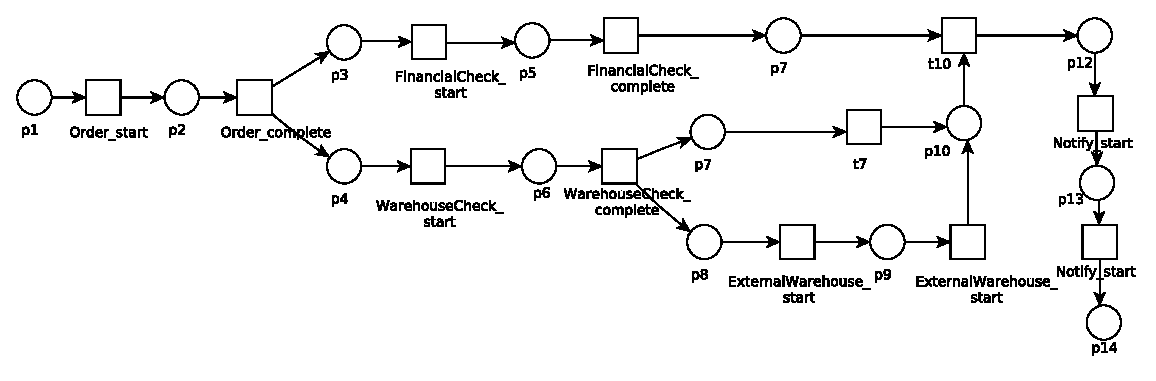
\includegraphics[width=360pt]
{./items/Sales_PN.pdf}
\caption{Petri net}
\end{figure}

L'esmepio scelto si ispira ad una procedura che trova applicazione all'interno di organizzazioni a carattere commerciale, si tratta del processo di vendita. In questa sede viene considerata solo una sua semplificazione rispetto a quanto avviene realmente. Per noi, il processo di vendita inizia con l'attività 'notify', in questa fase viene accolto un ordine da parte di un cliente. Dopo la ricezione dell'ordine, vengono condotte alcune attività in parallelo (visto che non presentano alcuna dipendenza tra loro) una di queste è l'attività 'FinancialCheck', in questa fase viene effettuata una valutazione dell'ordine dal punto di vista finanziario, possiamo ad esmepio pensare che vengono condotte delle indagini sulla solvibilità del cliente che ha emesso l'ordine. Parallelamente viene svolta l'attività 'ExternalWarehouse'...

\section{Conformance and Performance Analysis based on Petri nets}\label{Background}

The process analysis is performed by using the Petri net modelling the process and an event log recording the related executions (process instances). The basic building blocks of event logs are events. An event {\itshape e} can be seen as a pair {\itshape e = (a,t) } representing an action {\itshape a } recorded and the corresonding timestamp {\itshape t}. Action and timestamp are denoted respectively by $\alpha(e)$ and $\phi(e)$. Events that belong to the same process are grouped into {\itshape traces}. Formally, a trace $T$ is a finite sequence of events $T[1],..., T[n]$, such that $\phi(T[i]) \leq \phi(T[i+1])$ for all  $i \in [1,n)$. A log $L$ is a set of traces, recording the activities performed by a system during a finite number of process executions. We assume here the following hypothesis:
\begin{itemize}
\item All traces are instances of the same process.
\item For each action there exists a corresponding transition in the net that will be denoted, for simplicity, by the same name of the action.
\end{itemize}
The key algorithm expoloited to analyze the Petri net model with respect to the log is the {\itshape log repaly} algorithm. Given a Petri net model and an event log as intput to the algorithm, the output results can be used to check the conformance of traces and to evaluate some performance metrics. For each trace in the log, log replay starts by placing one token in the start place of the net. For each event in the trace the corresponding transition is fires in an {\itshape non blockin way} and the marking of the net is updated. ``Non blocking replay'' means that if the log replay execution requires to fire an enabled transition, the missing tokens are created artificially. The output of the log replay of a trace can be represented as an orderd list $R$ of pairs $(tr, i)$, representing that the transition $tr$ has been fired to mimic the event $T[i]$.
\\

In general, there could be exist some transition in the net called {\itshape invisible}. This can happen if the transition models an internal choice that is not visible in the system, or it is used to implement a construct of a more abstract modelling language (BPMN or others). Usually, invisible transitions are considered to be lazy, i.e, when firing a visible transition $t$ corrisponding to an event of the trace, only then the invisibile transition enabling $t$ is fired. However, in this paper, we adopt an other way for handling these transitions and the firing is performed as soon as possible. This allows to carry out some performance measures as explained that are not possible with the lazy metohode as explained in \cite.(riferimento al paper Applying Process Analysis to the italian eGov Entreprise Architecture)\\

The result of log repaly can be used to evaluate conformance and performance of the Petri net model. Conformance problems can be discovered by analyzing the tokens that have been artificially created {\itshape (the missing tokens)} and the tokens tha were not consumed {\itshape (the remaining tokens)}.\\

To clarify the conformance analysis technique we exploit the Petri net presented in section \ref{example} with reference to tow traces , $T$ and $T'$, presented respectively in figures \ref{ConfLog} and \ref{NonConfLog}. The log replay execution of the trace $T$, which is compliant with the Petri net, terminates with a marking containing one token in the end place \{${p14 \rightarrow 1}$\}, and returns the sequence:
\begin{equation}
\begin{split}
R&=\{(Order\_start,1), (Order\_complete,2),(WarehouseCheck\_start,3), \\
& (FinancialCheck\_start,4),(WarehouseCheck\_complete,5),\\
& (FinancialCheck\_complete,6),(t10, 6), (Notify\_start,7), (Notify\_complete,8)\}
\end{split}
\end{equation}
The log replay execution of the trace $T'$ terminates with remaing tokens \{${p8 \rightarrow 1,p14 \rightarrow 1}$\} and a missing token \{${p10 \rightarrow 1}$\}. The missing token is created artificially and this fact records a wrong execution of the event $Notify\_start$. In fact, notice that in the trace $T'$ this event is executed before the termination of the activity ``FinancialCheck'', and this is interpreted as a non conformance to the process model. The sequence returned by log replay is:
\begin{equation}
\begin{split}
R'&=\{(Order\_start,1), (Order\_complete,2), (WarehouseCheck\_start), \\
& (FinancialCheck\_start,3), (WarehouseCheck\_start,4),(t7,5), (t10,6)\\
& (Notify\_start,6), (Notify\_complete,7)\}
\end{split}
\end{equation}

\begin{figure}[t]\label{ConfLog}
\centering
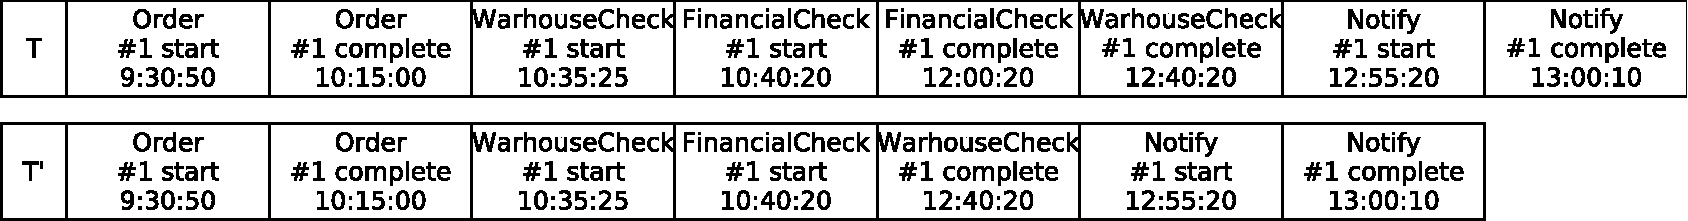
\includegraphics[width=400pt,height=40pt]
{./items/logConforme.pdf}
\caption{Conforme log example}
\end{figure}

\begin{figure}[h]\label{NonConfLog}
\centering
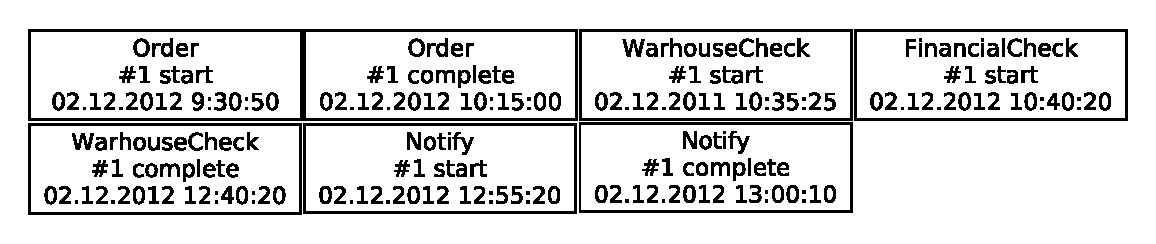
\includegraphics[width=400pt,height=40pt]
{./items/logNonConforme.pdf}
\caption{Non conforme log example}
\end{figure}

Since the logs contain timestamps, the log replay can be used to compute performance measures of the process. The idea is to calculate the time interval between production and consumption of tokens in each place. This tecniques can be applied only to traces that do not present missing token during the replay, because such tokens cannot have time information. During the log replay the following metrics can be computed for catch trace and each place:
\begin{itemize}
\item sejour time $(tsj)$ : the time interval between arrival and depature of tokens;
\item synchronization time $(tsc)$: the time interval between arrival of a token in the place and enabling of a transition in the post-set of the place;
\item waiting time $(tw)$:  the time interval between enabling of a transition in the post-set of the place and token departure (thus $tsj=tsc+tw $).
\end{itemize}

To clarify the metrics evaluated by this tecnique, as done with conformance analysis, we exploit the Petri net  presented in section \ref{example} and the trace T presented in figure \ref{ConfLog}. The replay starts with firing the transition $Order\_start$ at time $0s$, thus a token arrives at $p2$ at time $0s$. After $45 min$ the token in $p2$ is consumed and the transition $Order\_complete$ is fired, so $tw(p2)=45min$, and a token arrives at $p3$ and $p4$. At the time $1h:5min:25s$ the transition $WarhouseCheck\_start$ is fired, thus $tw(p4)=20min+25sec$ and a token is produced at $p6$. At the time $1h:10min:20s$ the transition $FinancialCheck\_start$ is fired and a token is produced at $p5$, so $tw(p3)=25min+20s$. After $2h:30min:20s$ from the replay start the transition $Financial\_complete$ is fired, hence we have $tw(p5)=1h+20min$ and a token is produced at $p11$. At time $3h:10min:20s$ the firing of the transition $WarehouseCheck\_complete$ is executed, so $tw(p6)=2h+4min+55s$ and token is produced at $p7$ and $p8$. At the same time the invisible transition $t10$ is fired and a token is produced at $p10$. At this point the transition $t10$ is enabled, so firing it is now possible and a token is produced at $p12$. Notice that $tsc(p11)=40min, tsc(p10)=0s$. At the time $3h:25min:20s$ the transition $Notify\_start$ is fired and a token is produced in $p13$, after $4min+4sec$ the trasition $Notify\_complete$ is fired and $tw(p13) = 4min+40s$.

An important performance measure is the activity execution time. This can be deducted from the waiting time in the places between the start and the activity complete transitions. For example, time execution for ``FinancialCheck'' is given by the waiting time computed for the place $p5: tw(p5)=1h+20min$.\\

It is worth noting that the synchronization time is greater than zero only for places which contain on their post-set transitions depending from other places. For the Petri net in figure \ref{pnet}, the only places which can have a synchronization time not null are $p10$ and $p7$. For instance, the sycronization time is greater than zero for $p10$ in the trace in figure \ref{ConfLog}. That means that, for this particular instance of the process, the branch with the occurance of the activity ``FinancialCheck'' is faster than the branch with activities relating the warehouse.

\section{An approach based on classification for conformance analysis}
%Supponiamo di avere un numero altissimo di esecuzioni relative al medesimo processo registrate in event log. Supponiamo anche che tutte queste esecuzioni siano state analizzate dal punto di vista della conformance per mezzo del log replay. L'algoritmo di analisi log replay si limita ad individuare come mostrato in sezione \ref{Background} quali sono i punti in cui si verificano errori di conformance, tuttavia, esso non fornisce alcuna informazione sulle cause che generano queste anomalie.\\

%Riuscire ad individuare anomalie è uno degli obiettivo fondamentali nell'analisi dei processi, avere un'idea su quali sono le cause che li generano lo è ancora di più. Questo infatti permette di capire anche come agire per apportare eventuali correzioni. 
 
%Perciò l'idea che ci ha guidato in questo lavoro consiste nel riuscire ad individuare nei dati contenuti negli event log, eventuali pattern che possono influenzare gli scostamenti rispetto al modello prestabilito. Questo infatti potrebbe aiutare nell'individuare le cause che stanno dietro agli scostamenti del comportamento reale del processo rispetto a quello atteso.

Employing data mining techniques for process analysis was already experimented by Van Deer Aalst in \cite{decision mining in business process}. In this article \cite{}, the idea consists in discovering how data attributes may influence the routing of case. The motivation that encourages this work consists in the presence of a huge ammount of data recorded in the event logs in the form of attributes that could contain implicit information. In this contribution, the same methodology is adopted to offer an additional tool for process analysts.\\

With the approach presented here, the goal proposed is discovering patterns or rules in the event logs data in corrispondence of which conformance errors, discussed in section \ref{Background}, occur. The goal is to conduct an investigation into data to discover the cause of conformance anomalies. Given the enormous quantity of data, the analysis is carried out with the classification, one of data mining techniques. In a classification problem, data is represented by a collection of records (called instances too), each of them is caracterized by a tuple $(\mathbf{x},y)$, where $\mathbf{x}$ is an attribute set, while $y$ is a special attribute called ``target attribute'' denoting the belowing class of the record. With this technique, the idea is learning a classification model that maps each attribute set $x$ to one of the predefined class labels $y$. See \cite{} for more information about classification.\\

Analysing data arising from event logs can be transformed into a classification problem. The data set can be derived from the process data, in particular, each instance data determines a record of the data set. For the process presented in section \ref{example}, a record is charaterized by the following attributes set: an instance identifier, a client identifier, the client typology with two possible values: new client and consolidated client, the sales manager responsabile for the order, the chief financial officier name who conducts the financial evaluation activities, the warehouseman name for the warehouse check activities, a supplier name in case of an external warehouse acitivity, and finally the result comunicated to the client for the order issued. The conformance result for the process instance provides an additional and important data which takes the role of the target attribute. All these attributes are discrete and contribute to formulate the data set presented in table \ref{tab:SaleData} of the classification problem.\\

\begin{table}[!h]
\scriptsize
\centering
\begin{tabular}{|p{0,8cm}|p{0,7cm}|p{1,5cm}|p{1,2cm}|p{1,2cm}|p{1,2cm}|p{0.8cm}|p{1,2cm}|p{0,5cm}|}
\hline OrdIde & CltIde & CltType & SalMan & FinOff & WrhsMan & SplIde & OrdResut & Conf\\
\hline
1 & 20 & consolidate & Marc & Alexander & Alex & 15 & positive & yes\\
\hline
2 & 700 & new & Johann & Mario & Alex & 04 & positive & yes\\
\hline
3 & 10 &consolidate & Mary & Robert & Alex & 15 & negative & yes\\
\hline
... & ... & ... & ... & ... & ... & ... & .... & .... \\
\hline
... & ... & ... & ... & ... & ... & ... & .... & ...  \\
\hline
\end{tabular}
\scriptsize
\caption{Data set}
\label{tab:SaleData}
\end{table}
\normalsize

Many classification models could be used for a classification problem. For our purpose we choose the decision tree model because of its simplicity and diffusion. In a decision tree, each leaf node is assigned a class label (a values of the attribute target). The non-terminal nodes, which include the root and other internal nodes, contain attribute test conditions to separate records that have different characteristics. In principle, there are exponentially many decision trees that can be constructed from a given set of attributes. While some of the trees are more accurate than others, finding the optimal tree is computationally infeasible because of the exponential size of the search space.  However, efficient algoritms have been developed to induce a reasonable accurate decision tree in a a reasonable ammount of time. These algorithm usually employ a greedy strategy that grows a decision tree by making a series of decisions about which attribute to use for partioning the data. One is Hunt's algorithm, which is the basic of many existing desicion tree induction algorithms, including $C4.5$ used for our purpose.\\

Using existing data mining tools for classification, it is possible to build a decistion tree as a classification model for the example presented here, based on data produced artificially just for examplary purposes: from the event log recorded, the attributes that characterized the process are extracted, and all the resources needed for the classification algorithm employed are produced. The decision tree resulted is presented in figure \ref{salesDecTree}.\\

\begin{figure}[h]\label{salesDecTree}
\centering
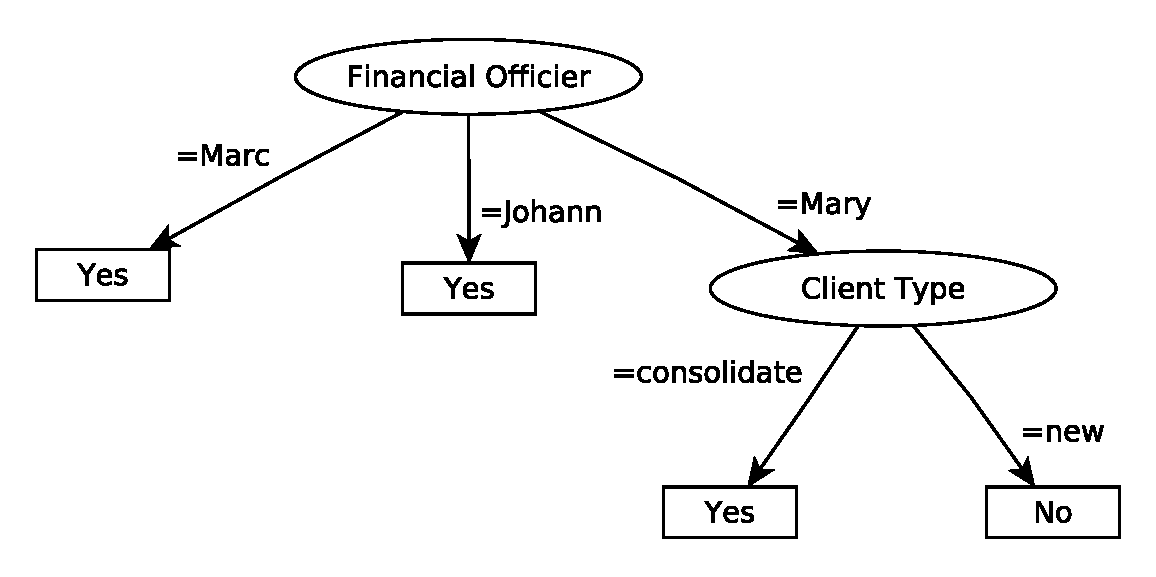
\includegraphics[width=230pt,height=110pt]
{./items/Sales_tree.pdf}
\caption{decision tree}
\end{figure}
The decision tree returned descibes a data pattern in corrispondence of which a process instance could present conformance errors: order managed by the sales manager ``Mary'' and received from consolidate clients of the organization may not respect the standard sales procedure. However, to get information most significant for our analysis, it is usefull to relate what is noticed by the decision tree and the log replay results. In figure \ref{replayResult} is presented a Petri net that resumes the conformance analysis conducted on instances recorded in the event log taken in exam. Arcs are labled by the number of activations done, red colored places presented missing or remaning tokens and colored transitions notice a wrong execution.\\
\begin{figure}[h]\label{replayResult}
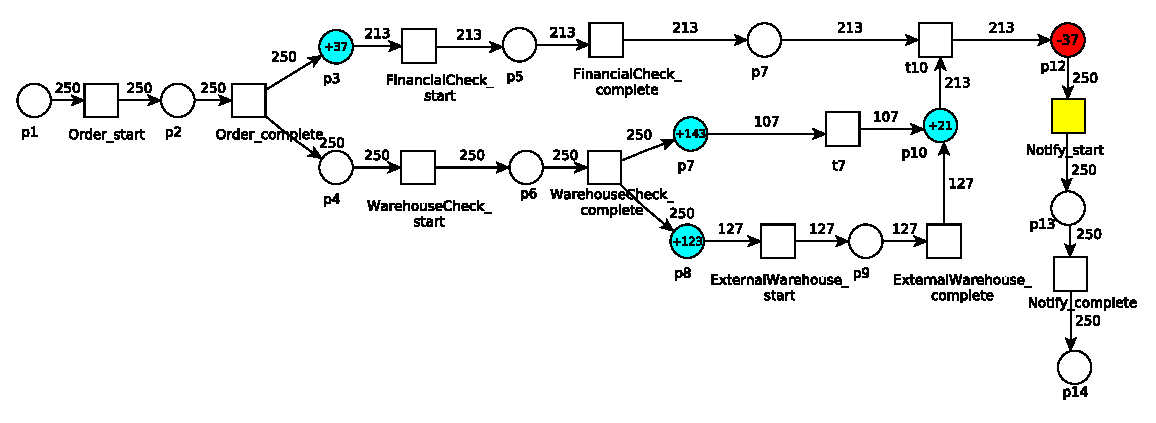
\includegraphics[width=390pt]
{./items/Sales_PN_result.pdf}
\caption{Petri net}
\end{figure}

The Petri net reporting the log replay results notice that there are 37 of 250 process executions with conformance erros, that is proved by the 37 missing tokens on the place $p12$ and a wrong execution of the transition ``Notify\_start''. In order to give an interpretation for this results, it must be taken into account the non blocking behaviour of the log replay. In this case, the 37 missing tokens in $p12$ notice that during the replay the algorithm needs to mimic the event ``Notify\_start'' but the transition associated to the event is not enabled in the marking reached by the net, so the algorithm creates artificial tokens for completing the trace repaly. This situation is possible only if the invisible transition $t10$ is not enabled. Now, if $t10$ is not enabled that means that there are no tokens in the place $p10$ and $p7$. But notice that there are 21 remaining tokens in the place $p10$, so the transition $t10$ is not enabled for those $37$ instances because the place $p7$ does not present tokens. Moreover, the Petri net in figure highlights 37 remaing tokens in the place $p3$, so we can deduce that in those instances financial activities were not performed. From this facts, we can conclude that the conformance problems presented in  37 instances are due to a missing execution of the Financial Activities check. On the other hand, the decision tree reports that the instances with conformance problems are made by consolidate clients. In this case, it might be reasonable that, for the orders made by the consolidate clients of the organization, could not be necessary a financial valutation of their situation.\\

Analysing the log replay results tanking into consideration patterns discoverd with classification technique leads to discover new cases to include in the process model by an extension. In other cases, if the process model is a representation of a fixed procedure to be respected, what discovered with such analysis can be used to take corrective measures. In fact, through a combination of the log replay results and the data patterns rules it may be possible to discover conformance errors cause, and this is fundamental to bring the right corrections. For instance, in the example presented here, if the model process represents a sales procedure that must be respected in any case, an appropriate correction can be taken to correct the wrong behaviour of the staff about consolidate clients. 


\end {document}
